\begin{figure}
    \centering
    \begin{subfigure}[b]{0.49\textwidth}
        \centering
        \begin{tikzpicture}
            \def\length{sqrt((x^2+y^2)^2  + (x*y)^2 )}
            \begin{axis}[
                    enlargelimits = false ,
                    view={0}{90},
                    xmin=0, xmax=1, ymin=0, ymax=1,
                    ytick distance=.125,
                    xtick distance=.125,
                    axis equal image,
                    grid=both,
                    major grid style={black},
                    axis equal image,
                    ticks=none
                ]
                \addplot3[
                    domain=.125:.875,
                    black,
                    quiver={
                            u={(x^2+y^2)/\length},
                            v={x*y/\length},
                            scale arrows=0.11
                        },
                    -latex,
                    samples=7
                ] {0};
            \end{axis}
            \begin{axis}[
                    enlargelimits = false ,
                    view={0}{90},
                    xmin=0, xmax=1, ymin=0, ymax=1,
                    xtick={.125,.5,.875},
                    ytick={.125,.5,.875},
                    axis equal image,
                    grid=both,
                    major grid style={red},
                    axis equal image,
                    ticks=none
                ]
                \addplot3[
                domain=.125:.875,
                red,
                quiver={
                        u={(x^2+y^2)/\length},
                        v={x*y/\length},
                        scale arrows=0.11
                    },
                -{Latex[length=3mm,width=3mm]},
                samples=3
                ] {0};
                \node  at  (axis cs:.125,.125)  [anchor=north west, red] {\(\hat{\mathbf{u}}\)};
                \node  at  (axis cs:.125,.333)  [left, black] {\(\mathbf{u}\)};
            \end{axis}
        \end{tikzpicture}
        \caption{Spline interpolation for the velocity field.}\label{fig:bsplinegrid}
    \end{subfigure}
    \vskip\baselineskip
    \begin{subfigure}[b]{0.49\textwidth}
        \centering
        \def\centerx{2}
        \def\centery{-1}
        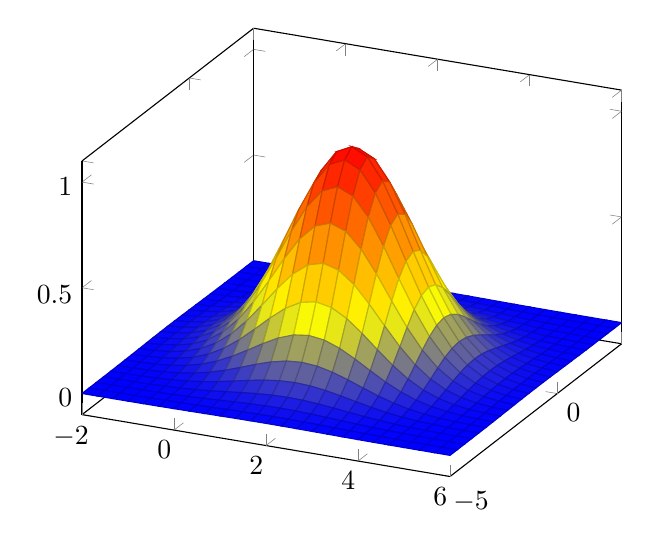
\begin{tikzpicture}
            \begin{axis}
                \addplot3[surf,domain=-2:6,domain y=-5:3]
                {exp(-( (x-\centerx)^2 + (y-\centery)^2)/3 )};
            \end{axis}
        \end{tikzpicture}
        \caption{Biquadratic spline basis function.}\label{fig:biquadspline}
    \end{subfigure}
    \caption{Spline interpolation for velocity fields.}
\end{figure}